In diesem Abschnitt wird auf den in \cite{hal02158423} vorgestellten, temporalen Algorithmus eingegangen.
Dieser besteht grundsätzlich aus dem \nameref{ch:Content2:sec:Sorting} sowie den 
\nameref{ch:Content2:sec:Retargeting}. Es sollte unbedingt beachtet werden, dass folgende
Annahmen getroffen wurden: Der Algorithmus arbeitet Blockweise auf den Pixeln und erwartet, dass benachbarte
Pixel innerhalb dieses Blockes den selben Wert haben. Da wir einen temporalen Algorithmus haben, soll diese Annahme 
auch über mehrere gerenderte Bilder hinweg gelten. Es sollte also beachtet werden, dass der Algorithmus z.B. nicht 
für Objektkanten oder ruckartige Bewegungen (der Kamera oder Objekte) ausgelegt ist.
Des Weiteren gehen wir aus den \nameref{ch:Content2:sec:a Posteriori} \textit{Eigenschaften}
gewonnen Einsicht, dass die Wahl 
unserer Anfangswerte des \nameref{ch:Content1:sec:Path Tracer} unsere 
Fehlerverteilung im Bildraum beeinflusst, aus. Somit werden wir ein Umsortieren
unserer Anfangswerte anhand einer blue noise Textur vornehmen, um so auch 
für die gerenderten Farbwerte der Pixel eine blue noise Fehlerverteilung zu 
erhalten. 

\par
\cite{bluenoisechrisschied} empfiehlt die Benutzung von $64^{2}$ 8-bit 
Texturen. Eine Benutzung in der Hinsicht, alle 64 bereitgestellten Varianten
in ein Array zu laden, jedes Frame ein neues Zufälliges zu verwenden und
mit einem zufälligen Offset drauf zuzugreifen. Die Database von Texturen 
\cite{bluenoisechrisschied} enthält für die empfohlene Auflösung jeweils
Varianten mit einer unterschiedlicher Anzahl von Kanälen. Wir wählen
die Anzahl der Kanäle anhand der Anzahl der Dimensionen, die gleichzeitig
blue noise verteilt werden sollen. Für unsere Variante reicht ein Channel 
einer Textur. Die gewonnen Einsicht bei \nameref{ch:Content1:sec:Quasi-Zufallsfolgen}
erlaubt uns eine Textur zu verwenden (und nicht eine Vielzahl von Texturen in ein
Array zu laden) und auf diese mit einem entsprechenden Offset zuzugreifen um 
entsprechenden Artfakten (Abrisskanten bei Bewegung, wiederholende Strukturen) 
vorzubeugen.
Abbildung \ref{fig:Path Tracer mit zufälligen Seeds} zeigt uns eine Szene mit zufällig 
gewählten Seeds und den daraus folgenden weißen Rauschen. Der Szenenausschnitt wurde
bewusst an einem homogenen Abschnitt gewählt. 

\begin{figure}[H]
    \begin{subfigure}{\textwidth}
        \centering 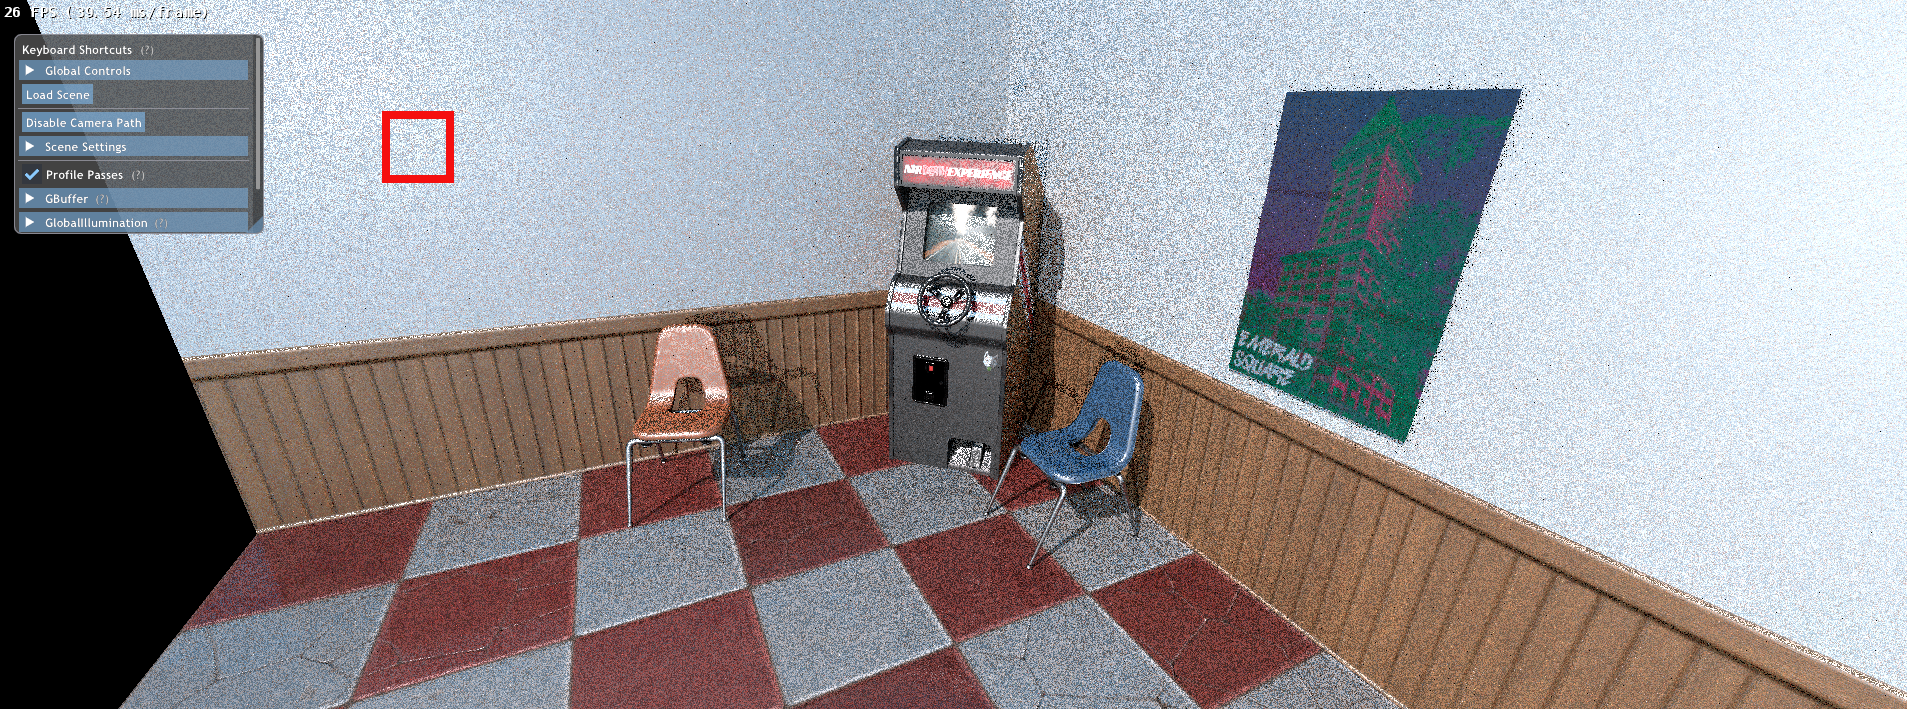
\includegraphics[scale=.2]{content/TemporalerAlg/Bilder/white_noise.png}
        \caption{Szene}
        \label{fig:Szene_Weißes Rauschen}
    \end{subfigure}
    \begin{subfigure}{0.5\textwidth}
        \centering 
\includegraphics[width=0.5\linewidth]{content/TemporalerAlg/Bilder/white_noise_64x64.jpg} 
        \caption{Szenenausschnitt}
        \label{fig:ausschnitt_Weißes_Rauschen}
    \end{subfigure}
    \begin{subfigure}{0.5\textwidth}
        \centering 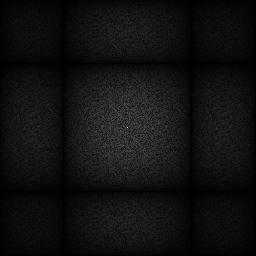
\includegraphics[width=0.5\linewidth]{content/TemporalerAlg/Bilder/white_noise_64x64_fourier.png}
        \caption{Fouriertransformierte des Ausschnitts}
        \label{fig:Fouriertransformierte_Weißes_Rauschen}
    \end{subfigure}
        \caption{Weißes Rauschen}
        \label{fig:Path Tracer mit zufälligen Seeds}
\end{figure}


